\chapter{Fault-tolerant design}

In this chapter, we introduce the concept of \emph{fault-tolerant design} -- a design paradigm in which the system is designed to tolerate certain types of failure during operation. In this chapter, we discuss:

\begin{enumerate}

 \item the notion of fault tolerance in systems, and its    link to reliability and high-integrity systems; and

 \item several design principles based on redundancy to design a    fault-tolerant system.

\end{enumerate}

\section{Introduction to fault-tolerance}
\label{sec:fault-tolerance:intro}

Recall from the subject \emph{Software Engineering Methods} that the reliability of   a system is expressed as a probability: it is the probability that a system may exhibit a failure over a defined interval. Reliability is often measured as \emph{Mean Time To Failure} (MTTF).

Despite our best efforts, faults will still remain in software once it is in operation. {\em Fault-tolerant design} is a body of principles and methods for designing systems so that they can continue functioning correctly in the presence of faults.

Fault-tolerant designs are used to achieve high reliability. By making a system more tolerant of faults, we increase the mean time to failure. Such an increase is important in many high-integrity systems. The higher the MTTF, the less chance there is of failure, making the system safer, more secure, or more reliable.


\subsubsection*{Definitions}

Before we start to discuss fault tolerance, we introduce some terms relevant to the topic, some of which you will already be familiar with; and some of which may be defined differently in other chapters in these notes (due to them being used in a different context/topic).

\begin{enumerate}

\item A \emph{failure} is a point in the functioning of a system where the
system behaviour deviates from its specification.

\item A \emph{fault} is an incorrect step, process or data definition which
will cause a system to fail for a given set of inputs.

\item An \emph{error} is a manifestation of a fault.

\item A \emph{hardware fault} is a physical defect that can cause a system or component to produce an error.

\item A \emph{software fault} is a defect in the source of the software that can cause a system or component to produce an error.

\item The \emph{reliability} of a system is the probability that the system will not exhibit a failure over a specified interval (e.g. time or set of inputs).

\end{enumerate}

\subsubsection*{Software and hardware failures}

It is important to note that \emph{software and hardware fail in different ways.}

Hardware can fail as a result of wearing of parts, or parts that were manufactured faulty. To repair the system, replacing the part with an equivalent part is generally sufficient. Further to this, hardware generally fails \emph{randomly}. In this context, ``randomly'' means that, given the same inputs, a hardware component can pass on these inputs one time, and then fail the next time. Hardware does not often fail as a result of a design fault.

Figure~\ref{fig:fault-tolerance:hardware-failure} shows a model failure curve for a hardware item. Hardware is likely to fail early due to a manufacturing error. If it does not, it tends to operate reliably for a period until the parts being to wear out, at which times its likelihood of failure increases.

\begin{figure}[!h]
\centering
  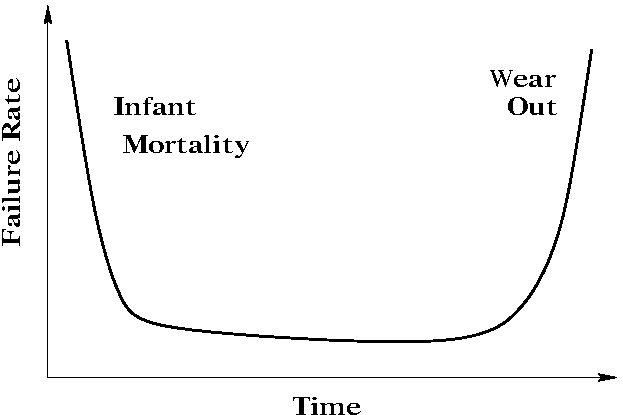
\includegraphics[scale=0.8]{\rootdir/fault-tolerant-design/figures/fault_hardware_curve}
  \caption{A model failure curve for hardware}
 \label{fig:fault-tolerance:hardware-failure}
\end{figure}

Software does not wear out. Failure are generally the result of the design, so replacing software will typically not restore the system. Further, software generally fails \emph{systematically}, meaning that in the same state, with the same inputs, it will fail every time, or success every time.

\subsubsection*{What is fault tolerance?}

 A system is said to be {\em fault tolerant} if it can continue to function according to its specification in the presence of a finite number of faults.

Thus, the field of fault tolerance accepts the fact that hardware and software will fail sometimes, but aims to produce a system that will be able to continue operating under a finite number of faults. In a fault tolerant system, the system itself must be able to detect that a fault has occurred, and work around it.


\subsubsection*{Classifying Failures}


There are generally accepted to be three main causes of failures:

\begin{enumerate}

\item Faults in the specification or design of the system. It is extremely difficult to assure the correctness of a specification. If the specification contains faults then everything that stems from it may also contain faults.

\item Faults in the components making up the system.
Components may be defective because of the manufacturing process or
because of wear and tear.

\item Faults due to environmental effects. Devices can be
subjected to a large number of environmental stresses, e.g. radiation
for space vehicles, temperature, or high G-forces. 

\end{enumerate}

\subsubsection*{Classifying Faults}


Faults may be classified using the following set of classes:

\begin{enumerate}

 \item \emph{Temporal behaviour classification}: There are essentially three types of faults:

 \begin{enumerate}[(a)]

   \item \emph{Permanent} faults do not die away with time but
      remain until they are repaired or the faulty component replaced.

   \item \emph{Intermittent} faults cycle between fault-active and      fault-benign states.

   \item \emph{Transient} faults die away after some time.

 \end{enumerate}

  \item \emph{Output behaviour}: There are two categories of output
behaviour:

  \begin{enumerate}[(a)]

   \item A task generates \emph{non-malicious} output if it is interpreted consistently by all processes receiving the output.

   \item A task generates \emph{malicious} (or \emph{Byzantine}) output if it cannot be interpreted consistently by all processes receiving the output.

  \end{enumerate}

  Byzantine faults are much harder to neutralise in practice. We will discuss this in detail in Section~\ref{sec:fault-tolerance:information-redundancy}.

  \item \emph{Independence and correlation}: Failures may be categorised as follows:

  \begin{enumerate}[(a)]

    \item \emph{Independent} failures do not cause other failures either directly or indirectly.

    \item \emph{Correlated} failures are sets of failures that are
related in some way.

  \end{enumerate}

\end{enumerate}


\subsubsection*{Redundancy}


The main means of ensuring fault-tolerance is through redundancy.  For a system to function despite the loss of some of its components means that there must have been spare capacity to begin with. 

Fault-tolerant design techniques can be divided into four categories:

\begin{enumerate}

\item \emph{Hardware Redundancy}: this involves multiple processors and
duplicate computations.

\item \emph{Software Redundancy}: this involves multiple developments of the
software. 

\item \emph{Information Redundancy}: this involves adding additional bits for error detection and recovery.

\item \emph{Time Redundancy}: this involves adding slacks to task schedules and rerunning tasks if necessary, which may required rolling back to correctly working states.

\end{enumerate}

The first three methods are the most commonly used in modern high-integrity systems, although the fourth is applied successfully in modern database systems. In this section, we will focus on the first three: hardware, software, and information redundancy.

Hardware and software redundancy are closely related --- the former inspiring the latter. However, due to the differences in how hardware and software can fail (as discussed above), techniques from hardware redundancy must be modified to be applied to software redundancy.

Throughout the rest of this chapter, we will look at some methods for achieve hardware, software, and information redundancy, and will analyse their effectiveness and limitations. 

\section{Hardware Redundancy}
\label{sec:fault-tolerance:hardware-redundancy}

The analysis of hardware is important in high-integrity systems. As discussed in Chapter~\ref{chapter:safety}, software on its own cannot cause physical harm --- it operates hardware that causes harm. 

The use of hardware redundancy is common-place outside of high-integrity systems. For example, the Google search engine is run on multiple servers to decrease the likelihood of users being unable to connect. However, we are especially interested in not just switching servers when a server goes down, but \emph{detecting and tolerating} specific faults in a system.



\subsection{Redundancy}


The use of redundancy for increase reliability is applied generally to electrical, mechanical, and software systems, however, the use of redundancy for reliability has been around for centuries:

\begin{quote}
``The most certain and effectual check upon errors which arise in the process of computation is to cause the same computations to be made by separate and independent computers; and this check is rendered still more decisive if their computations are carried out by different methods.'' -- D Lardner, 1824.
\end{quote}

The above quote is from D. Lardner's article in the {\em Edinburgh Review} from 1824. Lardner uses the term ``computer'' as it was 200 years ago: to refer to people who do manual calculations, rather than programs running on hardware.

Lardner's idea still stands today. To achieve fault tolerance in high-integrity systems, multiple units (hardware and/or software) are used to do the same calculations.

In 1824, if 2-3 ``computers'' were to calculate a result and find a different answer, the calculation would be re-done by all three, with the hope that the error made would not be repeated. However, when using hardware/software to do calculations, repeating the calculation is unlikely to result a different answer. Instead, different techniques are required to mitigate these problems.

\subsection{Static pairs}

A simple way to implement redundancy of hardware is to hard-wire two processors together to form a \emph{static pair}. The pair runs identical software using identical inputs and compares the output of each process.  If the outputs are identical then the pair is functional; otherwise it is deemed faulty and the interface switches the pair off from the network. This is a straightforward way to detect faulty processors/components.

\begin{figure}[!h]
\centering
  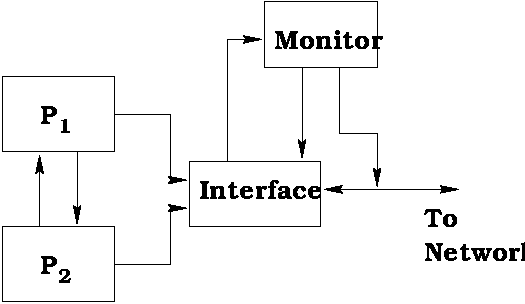
\includegraphics[scale=0.8]{\rootdir/fault-tolerant-design/figures/fault_static_pair}
\caption{Static pairing with a monitor}
\label{fig:fault-tolerance:static-pair}
\end{figure}


There are two assumptions in this:

\begin{enumerate}[(a)]

  \item that the interface does not fail; and

  \item that both processors do not fail identically and around
the same time. 

\end{enumerate}

Assumption (a) is not reasonable but assumption (b) is reasonable for hardware failures; that is, given reliable components, it is unlikely that both will fail identically at the same time.


The interface is a critical (single) point of failure of the pair. One way to mitigate this problem is to introduce an interface \emph{monitor} that checks the behaviour of the interface and conversely the interface can check the functioning of the monitor. Figure~\ref{fig:fault-tolerance:static-pair} presents a model of this. The monitor checks that if two different values are sent to the interface, the interface correctly switches the pair off the network. The interface checks the behaviour of the monitor as well. This introduces redundancy for the interface, so this cross-checking fails only if the monitor and interface fail at the same time.

\subsection{Redundancy and voting}

Static pairs can be used to detect a faulty component, however, they cannot continue operating reliably if one component fails, as there is no way to determine what the correct operating value should be. In the case of two redundant components, the best we can do when they disagree is to take some action such as shutting down to a fail-safe mode, because it is not straightforward (and often not possible) to determine which component has failed. As such, fault-tolerant designs tend to use \emph{more than two} redundant components.

Once more than two components are used, it must be determined which components are correct, and which are faulty. To do this, we can use {\em voting}. The basic method is to use multiple units (hardware and/or software) and to vote on the result.  The designer must decide whether to use \emph{exact agreement} or \emph{approximate agreement}.


\subsubsection*{Voting and consensus-based reliability}

Consider three processors \(A\), \(B\) and \(C\) such that \(A\) and \(B\) produce the value \(x\), while \(C\) produces the value \(x + \alpha\). The problem in voting-based solutions is:

\begin{quote}
 What is the value of \(\alpha\) which is acceptable?
 \end{quote}

If the same types of processors are executing the same code and receiving the same interrupts at the same time then it is easy to detect the faulty processor. If many components are in \emph{exact agreement}, and one or two are not, then we can be confident that the two that are not in agreement are faulty. However, this is often not the case.  \emph{Approximate agreement} arises more often. For example, fluctuations in sensor readings or using different processors and algorithms to eliminate design faults may produce slightly different readings, with no way to determine which is correct.

To mitigate this problem, we require a \emph{metric} \(d(x_1,\,x_2)\) to be defined on outputs \(x_1\) and \(x_2\). The metric is specific to the system being designed. Essentially, two value are said to be \emph{sufficiently equal} (SE) if and only if \(d(x_1,\,x_2)\) --- the difference between the two outputs --- is less than some specified error margin, $\epsilon$. That is,
\[ SE(x_1, x_2)~ \iff  ~ d(x_1,\,x_2) \leq \epsilon\]
However, the metric only provides us with a way to determine whether \emph{two} values are sufficiently equal. In voting, we must instead determine that many values (more than two) agree to determine an output value of which we are confident.

\begin{example}
Consider a system with two sensors used to read the temperature of a chemical storage tank. The reading is used to determine what action to take, such as lowering cooling rods into the tank. The system designers decide on an error margin of 0.2 degrees Celsius. The sensors then produce the readings 35.6 degrees and 58.0 degrees. There is no way to decide which reading is accurate, so no action can be taken. However, if we have three sensors, readings producing 35.6, 35.7, and 58.0 degrees respectively, then we can be quite confident (but not certain) that the reading of 58.0 is incorrect, so we can discard this value.

\end{example}

In the case of more than two components, we need a \emph{voting algorithm} to determine which readings are correct/incorrect. There are three common voting algorithms used in high-integrity systems:

\begin{enumerate}
 \item \emph{majority voting};
 \item \emph{generalised $k$-plurality voting}; and
 \item \emph{generalised median voting}.
\end{enumerate}

Each voting algorithm takes a set of values as input, which represent the outputs from the redundant components, and returns a single value based on those inputs, which can then be used by the system to make decisions.

\subsubsection*{Majority Voting}

The concept behind the majority voting algorithm is quite straightforward: the output is the value on which more than half of the components agree. However, this is not as straightforward to decide as it initially seems. For example, given the set of five sensor readings $\{30.1, 30.2, 30.3, 30.4, 30.6\}$, with an error margin of 0.2, what should the output be? The first two elements do not agree with the final element, and the last two elements do not agree with the first. The algorithm needs to provide a single value: which should be chosen?


Assume that there are \(N\) outputs to be voted on and that \(N\) is odd.  From an analysis of the system, we have chosen a metric and \(\epsilon\) such that \(d(x_1,x_2)\leq\epsilon\) if \(x_1\) and \(x_2\) are sufficiently equal for practical purposes (note that $d$ is not transitive).

The majority voting algorithm then proceeds as follows:

\begin{enumerate}

 \item From the set of inputs, construct classes of inputs, \(P_1\)\ldots\(P_n\), such that:

\begin{enumerate}[(a)]

\item \(x,y\in P_i\) iff \(d(x,y)\leq\epsilon\); and

\item \(P_i\) is \emph{maximal}; that is, if \(z\not\in P_i\) there there
exists a \(w\in P_i\) s.t. \(d(w,z) > \epsilon\).

\end{enumerate}

 Each class of values should therefore be a set of values that agree with each other, and any input that agrees with that set should be in that set. Values can appear in more than once class.

 \item Take the largest class, \(P_k\), generated. This represents the largest maximal set of inputs that agree with each other. In the case that there are multiple largest classes for the same size, break the tie arbitrarily.

 \item If \(P_k\)  contains more than \(\frac{N}{2}\) elements (that is, it forms a majority), choose any element in \(P_k\) as the output of the voting algorithm. Alternatively, one could take the average value.

 \item If \(P_k\) contains less than \(\frac{N}{2}\)  elements, the voting algorithm reports a failure --- no consensus could be reached. In such a case, the greater system must determine what to do, such as entering a fail-safe mode or raising an alert.

\end{enumerate}

So, the majority algorithms finds the largest set of values that agree with each other. If this forms a majority, then any value in that set is representative of the majority, and can be used as the voting algorithm output.

\begin{example}
Consider an example of an array of five sensors measuring the temperature of a chemical storage tank. The readings of the five sensors, and therefore the input to the voting algorithm are: 

\[30.1, 30.2, 30.3, 30.5, 30.7\]

The error margin is 0.2. None of the values can be immediately rejected, because each value agrees with at least one other value. Using the majority voting algorithm, we would allocate values to the following classes:

\begin{tabular}{llll}
& \(P_1\) & $=$ & 30.1, 30.2, 30.3\\
& \(P_2\) & $=$ & 30.3, 30.5\\
& \(P_3\) & $=$ & 30.5, 30.7
\end{tabular}

The class \(P_1\) is the largest class contains more than \(\frac{5}{2}\) elements, so any value will suffice. We select the middle value, 30.2, as the output.

\end{example}

\subsubsection*{Generalised $k$-plurality voting}

A generalised \(k\)-plurality voter is the same as a majority voter, except that the \(P_i\) that is chosen must contain at least \(k\) elements, where \(k\) is determined by the system designer, rather than simply \(\frac{N}{2}\) elements.

A majority vote is simply a generalised \(k\)-plurality voter with \(k = \frac{N}{2}\).

A \(k\)-plurality voter can be used to raise (increase \(k\)) or lower (decrease \(k\)) the risk tolerance of a system. That is, for a higher value of \(k\), meaning that a larger set must agree, the system designers are specifying that they will be less tolerant of failure, and therefore, they will be more risk averse. In most real applications, \(k\) is specified to be less than \(\frac{N}{2}\), meaning that a majority is not required.

\subsubsection*{Generalised median voting}

The generalised median voter is a straightforward mechanism that simply chooses the median value by continually removing the elements \(n\) and \(m\), such that for all \(i,j \in P\), \(d(n,m)\) is greater than \(d(i,j)\), until one element remains. Thus, it requires inputs that with a total order relation between them, such as $\leq$.



An {\em averaging} voter is not sufficient because even a single faulty unit can skew the results terribly. For example, consider a faulty unit that returns $0$ for all measurements, with two correctly functioning units. They may return \(0, 100, 102\). The average is \(67.3^*\), while the correct value is more likely to be around 101.



{\bf Question:} Couldn't the generalised median voting algorithm be even more influenced by faulty units: what if the median value is generated by a unit that is faulty?

\subsubsection{Comparison of voters}

Table~\ref{tab:fault-tolerance:voter-comparison} presents a comparison of the three voters for various situations. For example, if the outputs from all components are correct and sufficiently equal (the first row of the table), then all three voters will produce a correct output. However, if a majority of the outputs are incorrect and none are sufficiently equal (fifth row), then the majority and \(k\)-plurality voters will each produce no output, while the median voter will produce an incorrect output.

\begin{table}[!h]
\centering
\begin{tabular}{llll}
\toprule
{\bf Case} & {\bf Majority} & {\bf \(k\)-plurality} &
             {\bf Median}\\
  & {\bf voter} & {\bf voter} &{\bf voter}\\
\midrule
All outputs correct and SE\(^*\) & Correct & Correct & Correct\\
Majority correct and SE & Correct & Correct & Correct\\
\(k^{\dagger}\) outputs correct and SE 
         & No output & Correct & Possibly correct\\[3mm]
All correct but none SE & No output & No output & Correct\\
All incorrect and none SE & No output & No output & Incorrect\\
\(k^{\dagger}\) outputs incorrect and SE & No output & Incorrect & Possibly correct\\[3mm]
Majority incorrect and SE & Incorrect & Incorrect & Incorrect\\
All incorrect and SE & Incorrect & Incorrect & Incorrect\\
\bottomrule
~\\
\(^*\) SE = Sufficiently equal\\
\(^{\dagger}\) where \(k < \frac{N}{2}\)
\end{tabular}
\caption{Comparison of voter types.}
\label{tab:fault-tolerance:voter-comparison}
\end{table}

From this table, we can see some interesting aspects of the voters. Median voters always produce an output, so are useful in systems in which a decision must be made (e.g.\ there is no option to enter a fail-safe mode). Majority and \(k\)-plurality voters will only produce incorrect output in the unlikely event that there is a majority (or \(k\)-majority) that are all incorrect and sufficiently equal. Thus, these are used in systems in which taking the right decision is more important, and when the voter has no output, some alternative action (such as entering a fail-safe mode) is preferred.

\subsection{N-Modular Redundancy (NMR)}

The N-modular redundancy scheme is a method used for masking faulty components in  system.  It works by using multiple (N) redundant components (where N is usually odd) and voting on their output. There are two typical designs, outlined in Figure~\ref{fig:fault-tolerance:n-modular-redundancy}. This figure shows the popular \emph{triplex} design. The first design has one voter, while the second design has three voters, which mitigates the risk of the voter failing.


\begin{figure}[!h]
\centering
\subfigure[Triplex schema with 1 output]{
  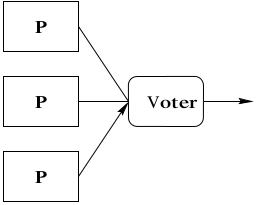
\includegraphics[scale=0.8]{\rootdir/fault-tolerant-design/figures/N-modular-redundancy-single-output}}
~~~~~
\subfigure[Triplex scheme with 3 outputs]{
  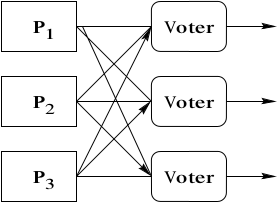
\includegraphics[scale=0.8]{\rootdir/fault-tolerant-design/figures/N-modular-redundancy-multi-outputs}}
\caption{Structure of a N-modular sub-system}
\label{fig:fault-tolerance:n-modular-redundancy}
\end{figure}

A system of \(N = 2m + 1\) components can tolerate \(m\) failed units. The most popular is the \emph{triplex} or \emph{triple redundancy} scheme, which can tolerate the failure of a single unit. For example, if a failure occurs in a triplex then the faulty unit can be detected next time there is a vote and the unit isolated.  This then forms a duplex that can detect a faulty unit, but it cannot mask it, because it is now similar to a static pair.

\begin{exercise}
With \(N\) units, how many failed units can N-modular redundancy tolerate to \emph{detect} a faulty unit, rather than \emph{mask} it?
\end{exercise}

\subsubsection*{Purging}

When a faulty unit is detected, it should be \emph{purged}, which means its results should no longer be considered, unless there is some reason to believe that the fault is transient. Purging can be done in two ways:

\begin{itemize}

 \item \emph{self-purging}, in which a unit compares its result to the voted output, and purges itself if it is sufficiently different; or

 \item \emph{\em sift-out redundancy}, in which all combinations of the pairs of units are compared with each other (producing a total of \({N \choose 2}\) outputs), and a controller can disconnect units that disagree with the majority.

\end{itemize}

While having multiple voters enables redundancy in the voters, there are other pragmatic reasons for  having multiple voters. Many applications may require only one output, however for others, multiple outputs may be sensible. For example, a braking system with four sensors (one on each wheel) to determine the current speed must also send four values to the four brake callipers. If one of the voters sends an incorrect value, the other three are still able to produce enough force for the car to brake at close to the correct speed. However, if one value is sent, and it happens to be incorrect, then the force applied may not brake the car.


\section{Software Redundancy}
\label{sec:fault-tolerance:software-redundancy}

Fault tolerance for software is harder than for hardware. While we can run software on multiple units of hardware, simply installing multiple copies of the software on redundant hardware does not mitigate software failures, because in general, the \(N\) copies of the software will all fail at the same time, caused by the same design fault.  These are called {\em common-mode} failures.

There are two general approaches used for software redundancy: \emph{N-version programming} and \emph{recovery blocks}. In this section, we present both of these in detail.

\subsection{N-Version Programming}

\emph{N-version programming} is a software-based version of hardware redundancy. The catch is that we cannot simply create N copies of the same software, as these will all fail on the same input. Instead, N-version programming requires that N \emph{independent} versions of the code are written.  All N independent versions of the code are executed and the output is voted on. Voting algorithms used in hardware redundancy can be used (e.g. majority voting).

However, careful planning and thought is required for this:

\begin{itemize}
 \item First, it will be considerably more expensive. For hardware items, the design is a big cost, but producing new hardware components is often relatively less expensive (compared to the design process).

 For software however, the effort in create new copies is essentially zero: copying some bits is so cheap as to not worry about the cost. The cost in software is all in the design. Thus, the effort to produce two independent software components is approximately double producing one.

 \item Second, it will not be effective if the same design and coding faults are replicated. It is well documented that if multiple separate software teams design, implement, and test the same system, they are likely to make mistakes in the same places as each other. Thus, we see common-mode failures in independent implementations of the same specification.

\end{itemize}


\subsubsection*{Common-mode failures}

Common-mode failures in engineering refer to those failures that are not statistically independent from one another. For example, the back two tires on a car a likely to fail (run out of tread) at around the same time because they will have driven the same distance.

In software, common mode failures typically result because programmers tend to make the same mistakes as each other; e.g. misinterpreting requirements in the same way, small boundary shifts, or or using the same (faulty) algorithm from a text book.

\subsubsection*{Causes of common-mode failures in software}

In software, common-mode failures can occur in multiple different implementations of the same system, irrelevant of operating environment or how long they have been in place. Common-mode failures can result in N-version systems due to  the following:

\begin{enumerate}

\item Faults in the original system specification. If two versions are implemented from the same specification, which contains a fault, then the two versions are likely to contain the same fault. In software redundancy, versions are often written from the same specification.

\item Development environments. Similar languages and environments encourage similar styles and similarity in programs, using the same programming tools may result in the same faults.

\item The use of similar algorithms. For example, different teams implementing the same numerical algorithm may implement the same instabilities, especially if they both use well-known algorithms for solving the problem.

\item Similar training to the independent teams. This is common within organisations.

\end{enumerate}


\subsubsection*{Eliminating common-mode failures}

Eliminating common-mode failures in N-version programming is done via introducing \emph{design diversity}. Essentially, this means implementing the same specification using diverse methods, tools, and teams.

In response to the four points in the previous section, common-mode failures can be eliminated using the following:

\begin{enumerate}

\item Eliminate as many faults as possible in the specification (easier said than done!).

\item Have a controlling individual who specifies the programming environments, languages, and tools that are used by the separate teams. That is, one person (or group of people) is responsible for ensuring that separate teams use diverse means for designing, implementing, and testing the software.

\item Keep development teams as separate as possible to avoid the use of common algorithms and data structures. This includes keeping them geographically separate to avoid them discussing their solutions with each other.

\item Use teams that have been educated/trained by different organisations. It is not uncommon to outsource to multiple organisations to introduce diversity.

\end{enumerate}


\subsubsection*{Design diversity through independence?}

Does using design diversity work? Unfortunately, statistics on these methods are hard to come by, because performing controlled experiments on large-scale systems is expensive.

One academic study performed by Knight and Leveson \cite{knight86} attempts to assess the impact of independence on common-mode failures. This study compared common-mode failures of student assignments implemented by individuals that were geographically separated. Overall, 27 different versions from two different universities were produced from the same specification: 9 versions from the University of Virginia (UVA) and 18 from the University of California and Irvine (UCI). The system was a simple missile defence system that took radar data as input and had to decide whether the signals represented incoming missiles. Neither set of students (from the different universities) were told that the other university was participating in the experiment, so it is unlikely that there was communication between individuals at different universities. 

All 27 versions were tested on the same 1 million tests, using the original version (produced by NASA) as the test oracle. Thus, the only faults that would not be noticed were those that failed on all 28 versions of the system.

Knight and Leveson compared the 9 UVA versions against the 18 UCI versions for common failures: that is, those that failed for the same test. The results are shown in Table~\ref{tab:fault-tolerance:correlated-failures}. For example, versions 3 and 11 both failed on the same 58 inputs as each other (out of a total of 1 million inputs).

\begin{table}[!h]
 \centering
 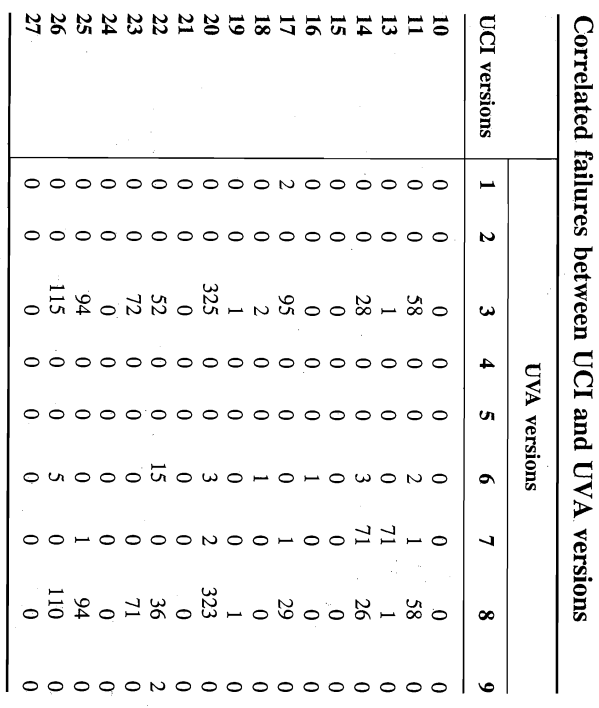
\includegraphics[scale=0.50,angle=90]{\rootdir/fault-tolerant-design/figures/correlated-failures}
 \caption{Results of the Knight and Leveson study on correlated failures}
 \label{tab:fault-tolerance:correlated-failures}
\end{table}

The results indicate that being part of independent teams is perhaps not enough to provide reliable results. For example, version 3 and 20 both failed on 325 of the 1 million outputs --- too high for a missile defence system.

Of course, from the results we can see that versions 3 and 8 are both particularly error prone; as are versions 20 and 26. These versions are probably less reliable than what we would expect from a team at NASA implementing a missile defence system. In addition, all versions used the same programming language. Nonetheless, the results indicate that independence alone may not be sufficient to achieve fault tolerance.

\subsection{Recovery blocks}

The \emph{recovery block} approach is similar to N-version programming in that it also uses N versions. However, only one version is executed at any one time. If the output does not pass an \emph{acceptance test} then next version is tried, and so on. Figure~\ref{fig:fault-tolerance:recovery-blocks} shows a schematic for this design pattern.

\begin{figure}[!h]
 \centering
 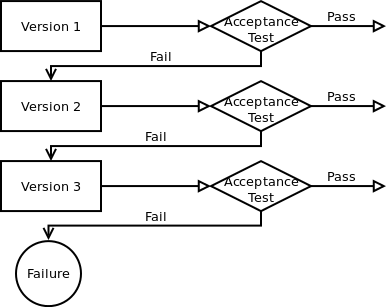
\includegraphics[scale=0.65]{\rootdir/fault-tolerant-design/figures/recovery-blocks}
 \caption{A schematic diagram for recovery blocks}
 \label{fig:fault-tolerance:recovery-blocks}
\end{figure}

When an acceptance test fails and another version is invoked, all changes to the state of the system must be reversed.

\subsubsection*{Acceptance tests}

Recovery blocks require \emph{acceptance tests} to determine whether the output is correct or not. This is the same as the {\em oracle problem} in testing.

Some acceptance tests can be straightforward to define; e.g. for example, a program that solves values for variables in an equation can be checked by substituting in the answer. Others, are more difficult and require something similar in complexity to the original program. For some problems, the complexity of checking a solution is considerably less than solving that problem, however, in many other cases, a {\em sanity check} is the best we can do.

\begin{example}
\label{ex:fault-tolerance:acceptance-test-gps}
As an example of an acceptance test, consider an algorithm that calculates the GPS coordinates of an unmanned vehicle to determine its location. Determining the position from GPS data is complex, however, estimating whether the location is correct based on other data can be reliable. For example, if the code performing the acceptance tests records the previous position from a few seconds prior, and knows the approximate speed and direction in which the vehicle is headed, then it can estimate the location using a simple ``dead reckoning'' algorithm.

Using such an algorithm, a small range of possible positions can be determined, and the output passes the acceptance test if and only if it falls inside that range.

\end{example}

The challenge with acceptance tests is to produce a tight but accurate range of possible values. If the designer attempts to be too accurate, this may result in a lot of false negatives --- that is, labelling an output as incorrect when it is in fact correct. If the design sets the range to loosely, this may result in a low of false positives --- that is, labelling an output as correct when it is incorrect.

The reliability of a recovery block is only as good as its acceptance test, so getting this right is of high importance. However, writing acceptance tests is more art than science.

\subsubsection*{Alternative versions in recovery blocks}

As with N-version programming, recovery blocks require diverse designs to mitigate common-mode failures, and so implementing the different modes is expensive. The question is then: \emph{why use recovery blocks instead of N-version programming}?

One reason is efficiency. The first version will generally be correct, so only one version will be executed. In addition, voting is not required.

However, a more pragmatic reason is development cost. Because the first version is likely to be correct, it will be executed the most. Similarly, if the first version fails, then the second version is likely to be correct as well, so the third version will hardly (if ever) be executed. As a result, one common strategy is to make each successive version more simple than the previous.

If the system can tolerate some outputs that are less accurate or are produced in a longer time, then an approximation algorithm or an algorithm with higher execution time may be much easier to develop. This has three benefits: 

\begin{enumerate}

 \item It reduces development costs, because each successive version should be easier and cheaper to implement than the last. For N-version programming, each version must be a ``full'' version.

 \item It introduces more design diversity between the versions. If the different algorithms are actually expected to produce different results, and may even take different inputs, then the diversity between the algorithms will be greater.

 \item The successive versions are more simple, which reduces the probability that there are faults. This increases the reliability of the entire block.

\end{enumerate}

\begin{example}
Consider the GPS algorithm for the unmanned aerial vehicle discussed in Example~\ref{ex:fault-tolerance:acceptance-test-gps}. We could implement two versions in a recovery block, and one acceptance test.

The first block uses the GPS data to calculate the coordinates, and, as in Example~\ref{ex:fault-tolerance:acceptance-test-gps}, a ``dead reckoning'' algorithm is used to determine a range of values for the acceptance test.

If the acceptance test fails, the dead reckoning algorithm is used to determine the \emph{most likely} location based on the previous location, the direction, and the speed. This is then used as the output.

 Most GPS devices use such a recovery-block approach to determining GPS location when they cannot receive a signal. Just check out your device the next time that you are in a tunnel with no GPS signal --- most devices will still attempt to track your current location.

\end{example}


\section{Byzantine Failures}

Note: See the lecture slides for details about this.

Recall from Section~\ref{sec:fault-tolerance:intro} that whenever a fault  causes multiple users of a unit to see different behaviour from that unit, the units is said to be behaving \emph{maliciously}. 

The idea of malicious output is a strange one, so let's illustrate it with an example. Consider a sensor sending out temperature readings to multiple components. If the communication mechanism between the sensor and the components is failing then, for each reading, each component may be receiving \emph{different} readings from the sensor. This is classed as a malicious or \emph{Byzantine} failure.

The term ``Byzantine'' comes from the \emph{Byzantine Generals' Problem}, proposed by Lamport et al.\ \cite{lamport82}.

\subsection{The problem}

When using multiple versions of a unit, having each unit receive a different reading from the source can effect the system. Consider the following table of readings from three sensors to three units, with sensor 1 being maliciously faulty and sending different numbers to the units:

\begin{center}
\begin{tabular}{llll}
\hline
 {\bf Sensor} & {\bf Voter 1} & {\bf Voter 2} & {\bf Voter 3}\\
\hline
 1 & 11 & 15 & 17\\
 2 & 14 & 14 & 14\\
 3 & 16 & 16 & 16\\
\hline
\end{tabular}
\end{center}

If we use a median vote, the outputs from the three sensors will be 14, 15, and 16 respectively. As such, there is no consistent decision between the units as to what the reading is, which may result in a failure of the system.

This is a serious problem in high integrity systems that requires addressing. As we will see, if a unit is failing maliciously, using the redundancy techniques presented in Sections~\ref{sec:fault-tolerance:hardware-redundancy} and \ref{sec:fault-tolerance:software-redundancy} often do not tolerate errors as expected. The example above demonstrates this.

As a result of this, Byzantine failures must be treated differently. In this section, we outline an algorithm for detecting that a Byzantine failure is occurring, and also for detecting which unit is failing.


\subsection{Byzantine Failures: The Canonical Example} 

To illustrate the method, we use the canonical example of the Byzantine army \cite{lamport82}.

Consider an army besieging a city. The army consists of the three commanders: the general \(G\)  and two lieutenants \(L_1\) and \(L_2\). All commanders are physically separated and can only communicate by two party messages. At most, one of the three commanders can be a traitor.  The messengers are assumed loyal. The group want to coordinate whether to attack or retreat, but can only communicate via the messengers.

If one lietenant orders his army to attack, but the other does not, the attacking army will be wiped out. Therefore, it is important that there is an agreement to attack or retreat.

\emph{Interactive consistency} is maintained if and only if:

\begin{enumerate}

\item All loyal lieutenants obey the same order.

\item If \(G\) is loyal then every loyal lieutenant obeys the order sent
by him.

\end{enumerate}

Treacherous behaviour violates the interactive consistency conditions. The problem is: can we detect a traitor in the group of commanders?

\subsubsection*{A traitor in our midst}

Consider the following schematic of a treacherous general attempting to make one lieutenant attack without the other:

\begin{center}
  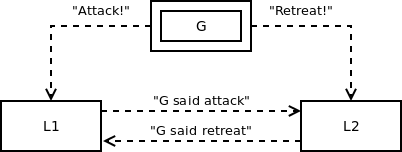
\includegraphics[scale=0.75]{\rootdir/fault-tolerant-design/figures/byzantine-3-party-general-traitor}
\end{center}

As we can see, the general is malicious in that he sends different messages to the two lieutenants.

The lieutenants can check the orders that they receive from the general to determine that they are consistent.  However, now consider the following example in which lieutenant \(L_1\) is a traitor, instead of the general:

\begin{center}
  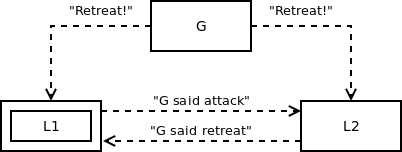
\includegraphics[scale=0.75]{\rootdir/fault-tolerant-design/figures/byzantine-3-party-l2-traitor}
\end{center}

From the perspective of \(L_2\), the messages it sends/receives are the same. It can detect that either the general or the other lieutenant is lying, but cannot decide which is lying, so cannot decide what to do. Thus the first condition of interactive consistency cannot be guaranteed, irrelevant as to whether the traitor is the general or the lieutenant.

The problem here is that traitors can lie about the message they receive (\emph{unless} they are using unforgeable digital signatures and message authentication).

What this scenario tells us is that, in the presence of malicious failure, the simple redundancy schemes do not work. That is, majority voting is not sufficient to find a faulty unit. While it can be detected that one unit is faulty, it cannot be detected \emph{which} unit is faulty, so interactive consistency cannot be maintained, and therefore, no consistent output is possible. The best we could do is report a failure and perhaps go into a fail-safe mode, but this is not a fault tolerant solution because the system does not continue operating under the failure.

\subsubsection*{A general with three lieutenants}

Next, consider the case where there are three lieutenants, and the general is treacherous. The table below outlines the messages that each participant can send to the other:

\begin{center}
\begin{tabular}{llll}
 \hline
  & \multicolumn{3}{c}{{\bf Received by}}\\
 \cline{2-4}
  {\bf Sent by}  & L1 & L2 & L3\\
\hline
 G & attack & attack & retreat \\
 L\(_1\) & - & attack & attack \\
 L\(_2\) & attack & - & attack \\
 L\(_3\) & retreat & retreat & - \\
 \hline
{\bf Majority vote} & attack & attack & attack\\
 \hline
\end{tabular}
\end{center}

All lieutenants can use a majority vote on the messages that they receive to coordinate the same action (provided there is only one faulty unit). Further, L\(_3\) knows that the general is the traitor, but  L\(_1\) or L\(_2\) do not, and L\(_3\) could not convince L\(_1\) or L\(_2\) of this.

Consider the case where there are three lieutenants, with \(L_1\) being treacherous. In this table, m$_1$ and m$_2$ are variables representing the fact they the value is irrelevant: the entry can be either ``attack'' or ``retreat''.

\begin{center}
\begin{tabular}{llll}
 \hline
  & \multicolumn{3}{c}{{\bf Received by}}\\
 \cline{2-4}
  {\bf Sent by}  & L1 & L2 & L3\\
\hline
 G & attack & attack & attack \\
 L\(_1\) & - & m$_1$ & m$_2$ \\
 L\(_2\) & attack & - & attack \\
 L\(_3\) & attack & attack & - \\
 \hline
{\bf Majority vote} & attack & attack & attack\\
 \hline
\end{tabular}
\end{center}

Again, using a simple majority vote on the messages that they receive,  interactive consistency can be maintained, irrelevant of the values of m$_1$ and m$_2$. We do not know who the traitor is, but we can still come to a consistent and correct outcome.

Therefore, by adding an additional lieutenant, we can not only detect that there is a traitor, but we can also mitigate the problem and choose the correct action (using voting). In the first examlpe, $L_3$ even knows who the traitor is.

\subsubsection{How many loyal commanders do we need?  How long does it take for them to agree?}

In the example with three lieutenants and a general, interactive consistency can be maintained in the presence of at most one traitor because there are enough messages to override anything the traitor does. But what about cases containing more than one traitor?

A general theorem is that to sustain interactive consistency in cases with \(t\) traitors, we require

\begin{itemize}
\item at least $t+1$ rounds of communication, and
\item at least \(3t + 1\) commanders in total.
\end{itemize}

\subsection{The Byzantine Agreement Algorithm}

The following algorithm \(Byz(n)\), where \(n\) is the number of traitors that must be sustained, can be used to maintain interactive consistency. The algorithm works by essentially have the lieutenants vote by treating each others' orders as votes:

\begin{quote}
Algorithm \(Byz(0)\)\\
\begin{enumerate}
\setlength{\itemsep}{0pt}\setlength{\topsep}{0pt}

\item The commander sends his orders to every lieutenant.

\item The lieutenant uses the order they receive from the commander or
the default (say retreat) if no order is received. 

\end{enumerate}

Algorithm \(Byz(n)\)\\
\begin{enumerate}
\setlength{\itemsep}{0pt}\setlength{\topsep}{0pt}

\item The commander sends his orders to every lieutenant. 

% Let \(v_i\) be the order sent to lieutenant \(L_i\).

\item For each \(i \in 1.. n\), lieutenant \(L_i\) acts as the general in a \(Byz(n-1)\) algorithm and sends out order \(v_i\) to each of the other \((n-2)\)  lieutenants, i.e.\ \((n-2)\) attempts to agree on \(L_i\ 's\) order.

\item For each \(i\) and \(j \not = i\), let \(w_{ij}\) be the order
that lieutenant \(L_i\) receives from lieutenant \(L_j\) in step 2
(using the \(Byz(n-1)\) algorithm), or the default if no order is
received.  Lieutenant \(L_i\) follows the majority \(\{v_i,
w_{i,j}|i\not = j\}\).

\end{enumerate}

\end{quote}

\subsection{Authenticated Byzantine Agreement}
The use of digital signatures to authenticate messages prevents traitors from lying about what they have received from others.  Using an authenticated version of the algorithm above, we can solve the Byzantine Agreement problem, tolerating $t$ traitors, in
\begin{itemize}
\item $t+1$ rounds of communication, 
\item with any number of commanders.
\end{itemize}

The $t+1$ rounds of communication are still necessary (this is also a theorem), but there is no longer a need to have many more honest commanders than cheaters.

\subsection{Byzantine failures in systems engineering}

\subsubsection*{Isn't this subject about systems engineering, not warfare?}

To relate this back to systems engineering, the commanders in the example are analogous to units in a system, and traitors are analogous to units that are failing maliciously. For  majority voting to work, inputs to the units must be consistent.

A simple mapping from the Byzantine generals' problem is to consider the general as a sensor, and the lieutenants as the redundant units receiving readings from the sensor that vote on the course of action. A treacherous general represents a faulty sensor, while a treacherous lieutenant represents a faulty unit (other than the sensor).

For systems in which we want to tolerate \(n\) malicious units sending inconsistent values, the Byzantine algorithm will ensure a consistent output that is decided if we have \(3n + 1\) units.

\subsubsection*{Byzantine algorithms in practice}

The \(Byz(n)\) algorithm above was first proposed by Lamport et al.\ \cite{lamport82}. For a long while, Byzantine fault tolerant schemes were considered too expensive to be practical, due to the number of messages and votes. However, the field of Byzantine fault tolerance was still of interest to a handful researchers, and in 2002, Castro and Liskov \cite{castro02} presented the ``Practical Byzantine Fault Tolerance'' (PBFT) algorithm, which provides a high performance algorithm for solving the problem of Byzantine failure.

The results shown by Castro and Liskov triggered a flurry of research on the topic, and now several high-performance and low-cost algorithms for Byzantine fault tolerance exist.

One recent example of Byzantine agreements/algorithms is the \emph{Bitcoin} system: a peer-to-peer system for digital currency. To obtain a single coin of currency, a node must work as part of a ``proof-of-work'' chain, and synchronisation of the global chain view is performed using a majority vote. However, malicious behaviour is clearly an obstacle, because there is an incentive to lie in an attempt to gain currency. A Byzantine fault tolerance algorithm is used to prevent this.

\section{Information Redundancy}
\label{sec:fault-tolerance:information-redundancy}

Information redundancy is one method for increasing the fault tolerance of a system. The basic idea behind information redundancy is to store/send more information than is necessary, and to use that extra information to check for errors, and in some cases, to correct errors.

Coding schemes are typically used to implement information redundancy. Network communications research and microprocessor research have resulted in some efficient methods that use information redundancy to detect corrupted data.

\subsection{Duplication}

{\em Duplication} is the most basic form of information redundancy: all information is duplicated. Errors can be detected by simply comparing each bit and its duplicate.

However, this requires twice as much storage/communication, requiring double the resources, so it is too inefficient to be implemented in most systems, especially real-time systems, or resource constrained systems, such as remotely operated vehicles.

Duplication can detect errors in information, but if the information is duplicated only once, then it cannot correct errors, because we cannot know whether it is the original or duplicate that is in error. To correct information errors, \emph{more than two} copies are required, which is a considerable overhead for many systems.

\subsection{Parity coding}

\subsubsection*{Error detection using parity coding}

{\em Parity coding} is a simple method for detecting 1-bit errors in information; that is, where 1 bit is incorrect.

It works by counting whether there is an odd or even number of 1s in an \(n\)-bit word, and then appending 0 (odd) or 1 (even) to the end of the bit. When this information is read, a check can be done by counting the bits in the first \(n\) bits of the word, and comparing the result to the \(n+1\)th bit. If these are different, then an error has occurred.

\begin{example}
The 8-bit word 00001111 is transferred over a communication channel between two nodes. There are an even number of 1s, so 9 bits are transferred: 000011111; with the final 1 indicating that there is an even number of 1s in the first 8 bits.

If one of the bits is corrupted, for example, the first bit (100011111), then the number of 1s is now odd. The receiving node counts the number of 1s in the first 8 bits, notices that this is odd, and compares this with the final bit, thereby detecting the error.

\end{example}

Clearly, parity coding only works if an odd number of bits have been corrupted. If two bits are corrupted, then the number of 1s will be the same as before.

Despite this, the simplicity of the method and the small overhead make it popular for information redundancy.

\subsubsection*{Error correction using interlaced parity coding}

\emph{Interlaced parity coding} is a parity coding method that can \emph{correct} as well as detect some bit errors. It works by dividing the word up into disjoint portions, and representing each portion with one bit --- again using 0 or 1 to represent whether there are an even or odd number of bits.

Table~\ref{fig:fault-tolerance:parity-coding}, taken from Krishna and Shin \cite{krishna99}, shows an example of this for an 8-bit word. Four parity bits are used, and depending on which parity bits are wrong, we can detect and correct one faulty bit, including if the parity bit is in error. In Table~\ref{fig:fault-tolerance:parity-coding}, the parity bits are associated with the bits using the following code:

\begin{itemize}
 \item $P_0$ covers bits $w_0, w_2, w_3, w_6, w_7,$ and $P_0$
 \item $P_1$ covers bits $w_0, w_1, w_3, w_5, w_6,$ and $P_1$
 \item $P_2$ covers bits $w_0, w_1, w_2, w_4, w_5, w_7,$ and $P_2$
 \item $P_3$ covers bits $w_0, w_1, w_2, w_3, w_4,$ and $P_3$
\end{itemize}

\begin{table}[!h]
\centering
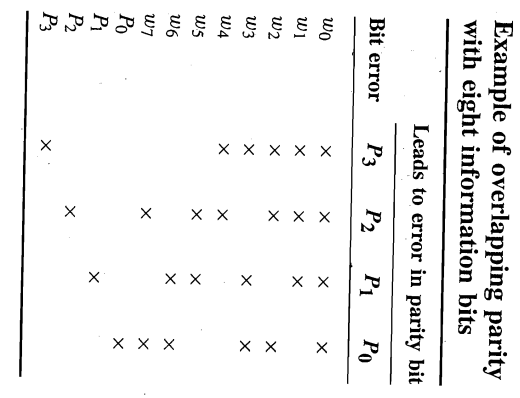
\includegraphics[scale=0.6,angle=91]{\rootdir/fault-tolerant-design/figures/extended-parity-coding}
 \caption{Parity coding for an 8-bit word, taken from Krishna and Shin \cite{krishna99}}
 \label{fig:fault-tolerance:parity-coding}
\end{table}

So, given an 8-bit word, the sender calculates the first parity bit ($P_0$) by counting whether there is an odd or even number of bits in the portion $w_0, w_2, w_3, w_6,$ and  $w_7$, and similarly for the other parity bits and their respective portions. It will then send a 12-bit word. The receiver can use this information to determine which (if any) bit is faulty.

Clearly there is an added overhead in this approach compared to the error detection technique discussed above, because it requires additional parity bits. As such, this scheme is generally only used in situations in which the original word cannot be recovered, such as storing information in memory or on disk. In cases where the word can be re-sent, error detection is generally sufficient.


\begin{example}
Consider an example of storing information in 8-bit words, with the additional 4 parity bits. One part of our program reads the stored word and parity bits: 00000000-1100. It must check whether the extended word is faulty.

It first calculates the expected value of the parity bits. The word is 00000000, so parity bits for this are straightforward to calculate: they are all 1 because there are an even number (zero!) of 1s in the string. As a result, the 12-bit word should be 00000000-1111.

There is no way of retrieving the original stored word, so the best we can do is try to correct this, hoping that a single bit is in error. Looking at the expected and actual parity bits, we see that bits $P_2$ and $P_3$ (the last two) are incorrect. By looking at Table~\ref{fig:fault-tolerance:parity-coding}, we can see that bit $w_4$ must be the faulty bit (assuming exactly one bit has been corrupted), because this corresponds to the row in the table in which only $P_2$ and $P_3$ would be in error.

Because we know that this is the faulty bit, and because we know it can take only one other value (the opposite bit value), we can correct the word to 00001000-1100.

\end{example}

\begin{example}
Consider the stored bits 00000000-1101. Again, we know that the parity bits should all be 1, so the bit $P_2$ is incorrect. Looking at  Table~\ref{fig:fault-tolerance:parity-coding}, we can see that the bit $P_2$ itself is the faulty bit. If we use the coding scheme shown in Table~\ref{fig:fault-tolerance:parity-coding}, then it is always the case that if exactly one parity bit is incorrect, then that bit is the faulty bit.

\end{example}

\subsection{Checksums}

The final information redundancy technique that we will look at is \emph{checksums}. Most readers are probably already familiar with the use of checksums in network messaging. Checksums are a useful error detection mechanism, but cannot correct errors.  Checksums are used to detect errors in blocks of data, especially when that data is being transferred between nodes.

The approach is simple. Given a block of data, break the data up into words; e.g.\ 32-bit words, and add these words together to get the checksum. The checksum is then appended to the data.

The receiver of the data strips the checksum upon receipt, re-calculates the checksum in the same way, and compares the re-calculated checksum to the stripped checksum. If they are different, the data has been corrupted.

There are a few different methods for adding together the words. The simplest is known as the \emph{longitudinal parity check}, which simply computes the \emph{exclusive or} of all words. To check the data, the sender simply computers the \emph{exclusive or} of all words \emph{including the checksum}. If the result contains a bit that is non-zero, then an error has been detected.

This can detect errors in multiple bits, but not if there are an even number of errors in the same bit of multiple words. The larger the set of blocks, the more likely it is to encounter an undetected error.

Checksums are popular because the overhead is small: for a block of 8-bit words, only an additional 8-bits are required. 



\section{Fault tolerance in practice}

\subsection{Airbus A310--A380}

The Airbus series of aircraft designs rely heavily on hardware, software, and information redundancy to achieve fault tolerant behaviour of aircraft. 

\begin{enumerate}

 \item A310 (circa 1983) had ten separate digital flight control computers.

 \item A320 (circa 1988) introduced fly by wire, in which four computers teamed in command/monitor pairs for redundancy, which became standard approach for subsequent Airbus flight control computers.

 \item A340 (circa 1992) had one command/monitor pair forming a ``fail fast'' module, failing over to another command/monitor ``hot spare'' pair.  Error detection was achieved through mismatched command, sequence checking, and self-test when aircraft energised.

 A second command/monitor pair using a different microprocessor and different software provided design diversity to tolerate common mode design and manufacturing faults.

 \item A380 (circa 2005) employs dual-redundant Ethernet for non-critical functions, electrical and hydraulic flight control diversity.

 Design diversity in the A380 project was achieved via using dissimilar computers, physical separation of teams, multiple software bases, different software development tools, and data diversity.

\end{enumerate}


\subsection{Boeing 777}

The Boeing 777 is another aircraft that relies heavily on hardware, software, and information redundancy.

\begin{enumerate}

 \item Goal of Mean Time Between Actions to 25,000 operating hours,
reduce probability of degrading below minimum capability to less
than \(10^{-10}\).

 \item Designed to tolerate Byzantine faults, object impact, component
failure, power failure, electromagnetic interference, cloud
environment.

 \item Byzantine fault tolerance with data synchronisation and median
voting.
 
 \item Architecture of flight control computer has three independent channels each composed of three redundant computing lanes (command, monitor, standby).  Standby allows dispatch of aircraft even with a lane or data channel failure.

 \item Design diversity was achieved using different microprocessor hardware and different software compilers for a fault-intolerant single source code.

\end{enumerate}




\section{Additional reading}

\begin{enumerate}

\item These notes were based mostly on Krishna and Shin's chapter ``Fault-tolerance techniques''  \cite{krishna99}, which is Chapter 7 in their book {\em Real-time Systems}.

 A PDF copy of Krishna and Shin's chapter is available on the LMS.

\item Moulding's chapter `` Designing for high integrity: The software fault tolerance approach'', which is Chapter 3 in C.\ T.\ Sennett, ed., {\em High-integrity Software}, Plenum Press, 1989 is a good resource of fault tolerance in high integrity systems. 

 The book is available in the library.

\item Laprie et al.'s article \cite{laprie90} titled ``Definition and analysis of hardware- and software-fault-tolerant architectures'' is an old but excellent overview of fault tolerance in systems engineering. It describes different techniques for achieving fault tolerance, including those outlined in these notes, and discusses their properties, such as cost, benefits, and limitations.

 A PDF copy of the article is available on the LMS.

\end{enumerate}



% LocalWords:  MTTF NMR GPS LMS Laprie iff Arlat Google llll Leveson
% LocalWords:  Beounes Kanoun UVA UCI Lamport et al unforgeable Byz
% LocalWords:  ij Liskov PBFT Bitcoin th Checksums checksums checksum
% LocalWords:  PDF
